\documentclass{report}
\usepackage{graphicx}
\usepackage{textcomp}

\usepackage{caption}
\usepackage{subcaption}

\newcommand{\tab}{\hspace*{1.5em}}

\begin{document}

\title{Practical 1: Modelling}
\date{\parbox{\linewidth}{\centering%
\textsc{Student ID: 120017875}\endgraf
\textsc{Module Code: CS4402}\endgraf
\textsc{Module Title: Constraint Programming}\endgraf
\textsc{Lecturers: Ian Miguel, Peter Nightingale}\endgraf
\today}}
\maketitle

\section*{Overview}
\tab This practical is centred around constraint modelling for M-queens puzzle. Firstly, two models corresponding to two different viewpoints of the problem are designed, and the design decisions are discussed in the first section of the report. These models are then compared to each other, and experiments are carried out with changing optimisation levels and trying out various heuristics to see how models perform under multiple different conditions. The results of these experiments are described in the second section. Finally, symmetry breaking constraints and constraints setting a lower bound for the number of queens necessary, and their according improvement on the model performance are discussed in section three.

\section*{Models of M-Queens puzzle}
\tab M-Queens puzzle is a variation of Queens Problems. Problems of this type ask you to find a way of placing a number of queens on a chess board so that certain conditions are fulfilled. In the case of M-Queens, there are two conditions - independence and dominance. Independence requires the queens to be placed in such a way that no two queens attack each other, while dominance requires all the cells of the chess board to either be attacked by some queen(s) or occupied by a queen.

I will now discuss two different viewpoints of M-Queens -- two different ways of representing a chess board with queens on it, and the constraints placed upon them.

\subsection*{0/1 model (part 1)}
\tab This is a very intuitive way of representing a chess-board. It is modelled as a two-dimensional matrix, indexed from \textit{1} up to \textit{M} (where \textit{M} is a parameter specifying the board size, and thus giving an instance of the M-Queens problem class). Each cell of the matrix is assigned either a value 0 or 1, where cells with 1 correspond to squares with queens on them, and cells with 0 correspond to empty squares. Figure 1. displays a solver output for a 4*4 chess board, and its correct interpretation.

\begin{figure}
\begin{subfigure}{.5\textwidth}
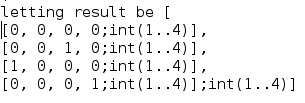
\includegraphics[scale=0.65]{images/p1.png}
  \label{fig:sub1}
\end{subfigure}%
\begin{subfigure}{.5\textwidth}
\hspace{2cm}
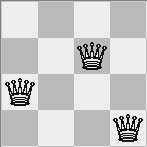
\includegraphics[scale=0.65]{images/p1_vis.png}
  \label{fig:sub2}
\end{subfigure}
\caption{An example of 0/1 model output and its interpretation on a chess board.}
\label{fig:test}
\end{figure}

The two constraints can then be checked accordingly:
\begin{itemize}
\item \textbf{Independence:} require every column, row and diagonal to have no more than one queen placed on it. This can be obtained by requiring the sum of elements of each column, row and diagonal to be less than or equal to 1. For rows and columns it is very straight forward -- use the matrix slicing operation to loop through row and column slices, requesting the sum in each to be less than or equal to one. With diagonals things are slightly more complicated, as they are more difficult to express. For diagonals going "upwards" ("/"), I used the fact that for each element of the diagonal its row and column indexes sum up to the same number. To obtain  diagonals going "downwards" ("\textbackslash "), I created a formula that picks out the necessary elements. The idea remains the same -- loop through diagonals, requiring the sum of each to be no more than 1.
\item \textbf{Dominance}: each square is uniquely identified by its row and column indexes. Therefore I use a double loop, where the outer loop goes through rows and the inner one -- through columns, to look at all the squares. I then check for each square individually whether it is under attack. For square to be under attack there must be a queen on either its row, column or one of the diagonals. Therefore for each square I require the sum of the elements of these to be bigger or equal to one (it is allowed for a square to be under attack by multiple queens or contain a queen, in which case the sum will equal 4).
\end{itemize}

\subsection*{My own	model (part 2)}
\tab The 0/1 model described previously is an explicit/occurrence model, while the model I designed is an explicit/explicit model. It is an indexed (\textit{1} to \textit{M}) one-dimensional array, where each cell gets assigned a number from \textit{0} to \textit{M} (where \textit{M} is the board size). Each cell can be interpreted as representing a column, where its content stands for the row number in which there is a queen. Say, if the third array element had a value \textit{6}, it would mean that there is a queen on the sixth row of the third column. If, however, an element takes the value of the dummy variable \textit{0}, it means that there are no queens in this particular column. This thus is an unambiguous way of uniquely representing a placement of queens on a chess board.

Figure 2. displays a solver output given this model for a 4*4 chess board, as well as its interpretation. Notice how this model provides a different (yet still correct) solution for a 4*4 board compared to the solution found by 0/1.

\begin{figure}
\begin{subfigure}{.5\textwidth}
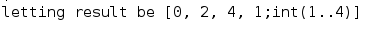
\includegraphics[scale=0.65]{images/p2.png}
  \label{fig:sub1}
\end{subfigure}%
\begin{subfigure}{.5\textwidth}
\hspace{3cm}
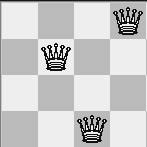
\includegraphics[scale=0.65]{images/p2_vis.png}
  \label{fig:sub2}
\end{subfigure}
\caption{An example of explicit/explicit model output and its interpretation on a chess board.}
\label{fig:test}
\end{figure}

Now about the constraints:
\begin{itemize}
\item \textbf{Independence:} once again, we have to show that there is no more than one queen in each row, column and diagonal. For columns, it follows directly by the design -- it simply is not possible to assign more than one queen for a column. For rows, I use the allDiff constraint to force all of the array elements (except for 0) take different values. For the upwards diagonal I take the same approach as previously -- note that queens with row and column indexes summing up to the same value are on the same diagonal, and force these sums to be all different. For downwards diagonals, I use the fact that the for two elements to be on the same diagonal, the difference between their row indexes and between their column indexes must be the same. So I check whether this is not the case for any two diagonals.
\item \textbf{Dominance}: similarly as for the first model, I loop through all squares of the chess board, and check whether there either is a queen on the square or the square is under attack. For columns, I look at whether the particular column has been assigned anything else but zero. For rows, I check whether the particular row index has been assigned to any column. For diagonals, I treat them in the same way as described before for the downwards ones.
\end{itemize}

\section*{Model comparison and experimentation}
\tab In this section I compare how my models perform relative to each other, and how various run parameters impact the solver. To simplify the process, I wrote a little bash script that automatically runs the solver with various parameters and extracts the necessary information (getResults.sh).

\subsection*{0/1 vs explicit/explicit}
\begin{figure} [\textwidth]
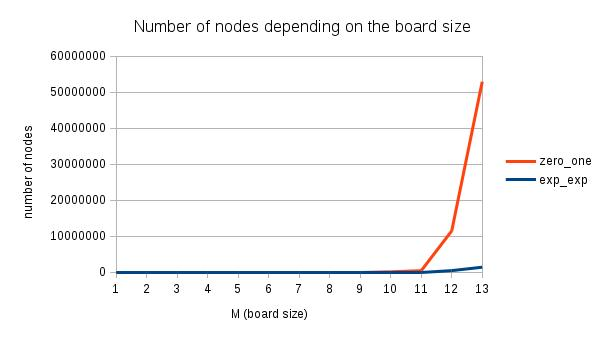
\includegraphics[scale=0.7]{images/numNodes.jpg}
\caption{Increase in the number of nodes created relative to board size.}
\end{figure}

\begin{figure} [\textwidth]
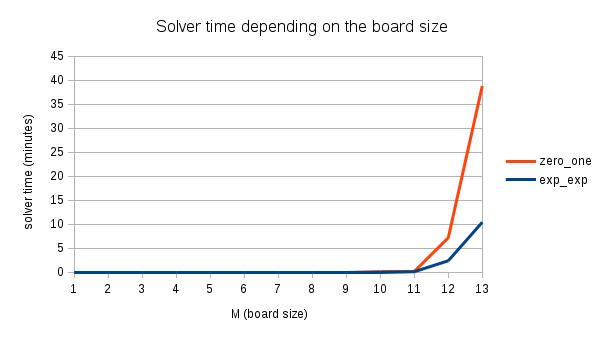
\includegraphics[scale=0.7]{images/solverTime.jpg}
\caption{Increase in the solution time relative to the board size.}
\end{figure}
\tab I found that in general my explicit/explicit model performs much better than the 0/1 model, which is especially visible when it comes to chess boards of size 10*10 and above. For both models the number of nodes and the time it takes to find a solution grows exponentially relative to the board size. I ran my explicit/explicit model for 15*15 board, and that took a little above 5 hours. Taken the relatively poor performance of 0/1 model, I did not even attempt such a big board for it. The increase in the number of nodes used is displayed in figure 3., while the increase in the time taken to find a solution is displayed in figure 4.

Interestingly, we can see that the number of nodes created does not directly correlate to the solution time. It is visible both -- from the figures 3. and 4., where number of nodes used by 0/1 model grows much faster relative to explicit/explicit model than the solution time taken, as well as from the results regarding heuristics and optimisation that are discussed later.

\newpage

\subsection*{Optimisation levels}
\tab Interestingly, varying optimisation levels provided contrasting results for the two models. I looked at how optimisation levels impact the number of nodes created, the time taken to solve the problem as well as the time taken by Savil Row to optimise it. I ran tests for all optimisation levels (0 to 3) for both models for board sizes from 1 to 11. Here are the results:

\begin{figure} [\textwidth]
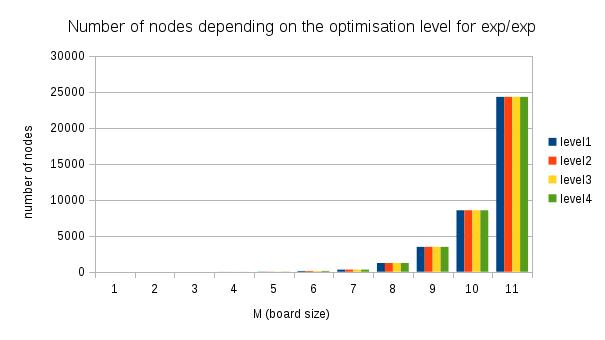
\includegraphics[scale=0.6]{images/optim_p1_nodes.jpg}
\caption{The number of nodes created for the explicit/explicit model for various optimisation levels.}
\end{figure}

\begin{figure}
\begin{subfigure}{.5\textwidth}
\hspace{-4cm}
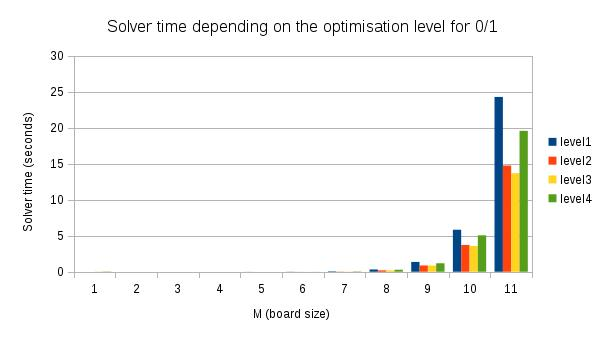
\includegraphics[scale=0.47]{images/optim_p1_solverTime.jpg}
  \label{fig:sub1}
\end{subfigure}%
\begin{subfigure}{.5\textwidth}
\hspace{1cm}
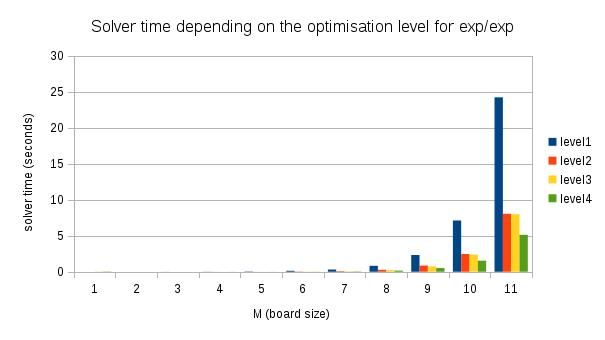
\includegraphics[scale=0.47]{images/optim_p2_solverTime.jpg}
  \label{fig:sub2}
\end{subfigure}
\caption{The solver times depending on the optimisation levels for both models.}
\label{fig:test}
\end{figure}

\begin{figure}
\begin{subfigure}{.5\textwidth}
\hspace{-4cm}
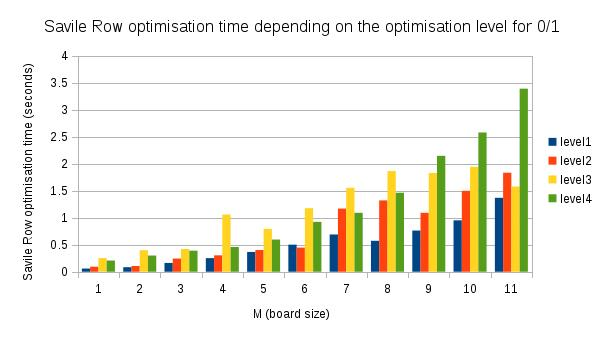
\includegraphics[scale=0.47]{images/optim_p1_srTime.jpg}
  \label{fig:sub1}
\end{subfigure}%
\begin{subfigure}{.5\textwidth}
\hspace{1cm}
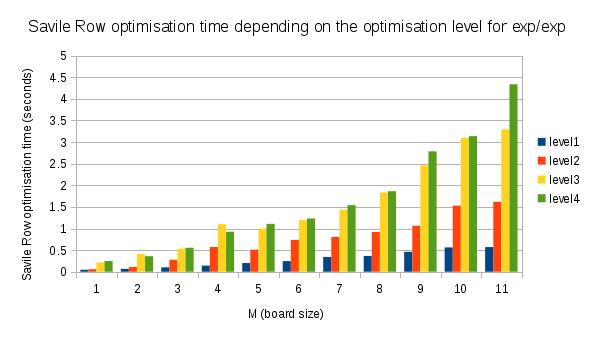
\includegraphics[scale=0.47]{images/optim_p2_srTime.jpg}
  \label{fig:sub2}
\end{subfigure}
\caption{The solver times depending on the optimisation levels for both models.}
\label{fig:test}
\end{figure}

\begin{itemize}
\item \textbf{Number of nodes:} optimisation levels had very little impact on the number of nodes used for both models. For the explicit/explicit model there was no change at all, as can be seen in figure 5. While for the 0/1 model the number decreased by a very small magnitude. This also speaks for the observation that solver times and the amount of nodes are not directly linked, as the solver times are strongly influenced by the optimisation level.
\item \textbf{Solver time:} the change in this was the most interesting. As it could be predicted, for explicit/explicit model the higher the optimisation level, the faster the solver is. There is a big jump between no optimisation and level 1, and a smaller one between level 2 and level 3. In general, the highest optimisation level provided solution about five times faster than when no optimisation was used. This is in a strong contrast to the results provided by the 0/1 model, where O0 and O3 levels have almost the same performance, while O1 and O2 are slightly better. I can only explain this by constraint propagation taking more time than branching would, when some more sophisticated optimisation methods are added.  Figure 6. provides a graph summarising the results.
\item \textbf{Savil Row optimisation time:} both models show that the higher the optimisation level, the more time it takes to perform the according optimisations. This is illustrated in Figure 7. Interestingly though, for some board sizes (especially M=4) level 1 optimisations take longer than level 3 ones, which is counter-intuitive, taking that level 3 is supposed to do everything that level 1 does and more.
\end{itemize}


\subsection*{Using heuristics}
\tab I also tried to impose various heuristics on both models. For both of them there is only one decision variable, thus the heuristics regulated branching on the search tree of it. I tried pushing branching on diagonals, rows or columns first, but somehow could not get the syntax right and the code did not get parsed.

Here are the results that I obtained by using various heuristics:
\begin{itemize}
\item \textbf{static and sdf:} did not make any difference for either of the models. I am guessing that it is because "static" is the default heuristic, while "sdf" branches on the smallest domain first, which does not change anything when only one variable is considered.
\item \textbf{conflict:} this heuristic worked very well for my explicit/explicit model. With the highest optimisation level it decreased the number of nodes by an order and decreased solving time by two thirds. Interestingly, it also decreased Savil Row optimisation time by a third. However, for the 0/1 model the number of nodes decreased only marginally, and so did the solution time.
\item \textbf{srf:} this heuristic did not provide good results for either of the models. For the 0/1 model nothing much changed, while the time results for the explicit/explicit model were slightly worse compared to default, and the number of nodes was increased almost twice.
\end{itemize} 

\section*{Model improvement by adding additional constraints}

\tab I researched two additional ways of improving the models by imposing extra constraints. 

\subsection*{Lower Bound}

Firstly, it turns out that there is a mathematically proven lower bound on how many queens are necessary to satisfy the M-Queens problem. This has been shown to be $\lfloor \frac{M}{2} \rfloor$ \cite{EJC}. It has also be shown that for boards of size M, where M can be expressed as \textit{4k+1}, the lower bound is \textit{2k+1} \cite{GW} (strictly larger than the other one). Both of these results have been shown for queens domination problem where the independence constraint has not been imposed (queens can be attacking each other). However, any solution for independent domination problem is also a solution of domination problem, thus the bound holds for both. Imposing a lower bound for the number of queens significantly speeds the solver up, as board combinations with fewer queens will not be considered, thus decreasing the search tree (and number of nodes used).

\begin{figure} [\textwidth]
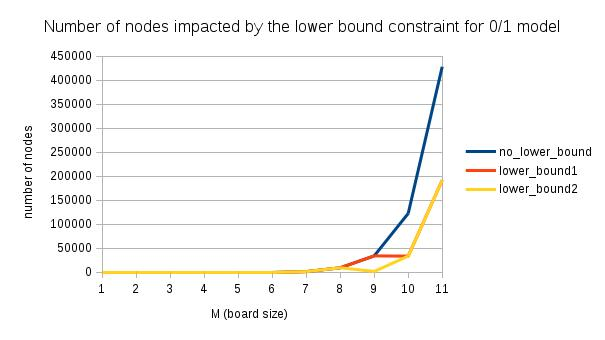
\includegraphics[scale=0.6]{images/p1_LB.jpg}
\caption{The impact that using a lower bound has on the number of nodes created by the solver. The blue line corresponds to no bound constraints, the orange one -- to a model taking into account only the first constraint mentioned, while the yellow one -- to a model employing both constraints stated above. Notice the difference between the yellow and the orange lines where M = 9.}
\end{figure}

As can be seen in Figure 8., for the 0/1 model using a lower bound constraint decreases the number of nodes used by more than a half. We can also see how for M = 9 (which can be expressed as 2*4+1) using the first lower bound stated provides worse results than using the second bound. The time taken by solver decreases similarly, while the time taken by Savile Row decreases only marginally. Interestingly, when optimisation level 0 is used, there is no decrease in the number of nodes, yet the solver is still slightly faster when the additional constraints are employed.

Cockayne \cite{EJC} also provides an upper bound for the number of queens necessary, yet I found that adding it did not decrease the number of nodes. I am guessing that the solver automatically explores the smallest possible options first because of the minimising constraint.

\subsection*{Symmetry}

Secondly, it can be observed that chess board has a very symmetrical structure. In fact, there are seven different symmetries that apply to it: symmetries to x and y axes and to both diagonals, as well as rotational symmetries by 90$^{\circ}$, 180$^{\circ}$ and 270$^{\circ}$ \cite{SPG}. Thus each solution of the M-Queens problem potentially has multiple other solutions in its symmetry class (while not necessarily, as it can be the case that applying symmetries produce identical solutions, for example, in the case of the trivial [1] solution to 1*1 board). It would be preferable to set constraints on the solver so that it would consider only one solution of each class, thus restricting the branching factor, as no-solutions symmetrical to other no-solution would not be explored. One has to be careful, however, not to eliminate all solutions of a symmetry class, as then it could be the case that solver produces no solutions to the problem at all.

\begin{figure} [\textwidth]
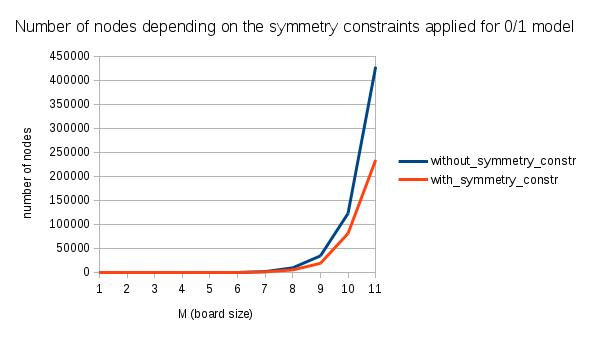
\includegraphics[scale=0.6]{images/p1_sym.jpg}
\caption{The impact that additional symmetry constraints have on the number of nodes constructed for solving the 0/1 model.}
\end{figure}

Thus I came up with the following symmetry breaking constraints (breaking five out of seven symmetries) for the 0/1 model:
\begin{itemize}
\item \textbf{Symmetry to x axis:} the idea is to require the first queen on the top half of the board to be in a lexicographically higher position or in a higher row that the first queen in the bottom half of the board (perceived from the bottom). I use lexicographical ordering to ensure this. 
\item \textbf{Symmetry to y axis:} similarly, we want the first queen on the left side of the board to be in a lexicographically higher position than the first queen on the right side of the board (when perceived from right to left). Once again, lexicographical ordering comes into play.
\item \textbf{Rotational symmetry by 90$^{\circ}$:} require the row with the first queen to be lexicographically bigger than the corresponding column by 90$^{\circ}$ rotation. Say, if it was the k-th row, we would compare it to the M-k+1 column.
\item \textbf{Rotational symmetry by 180$^{\circ}$:} require the row with the first queen to be lexicographically bigger than the corresponding row from the bottom, taken in the reverse order.
\item \textbf{Rotational symmetry by 270$^{\circ}$:} require the row with the first queen to be lexicographically bigger than the corresponding column by 270$^{\circ}$ rotation. Say, if it was the k-th row, we would compare it to the kth column, taken in a reverse order.
\end{itemize}

\begin{figure} [\textwidth]
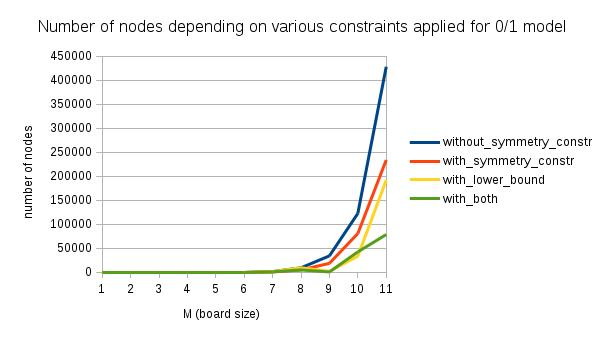
\includegraphics[scale=0.6]{images/allConst.jpg}
\caption{Comparison on the number of nodes when applying no, either or both of the additional constraints.}
\end{figure}

The additional constraints definitely do cut down on the symmetries -- for a 4*4 model, there are 16 solutions without symmetry constraints, and only 4 when the constraints are applied. In Figure 9. it can be seen that the current symmetry constraints reduce the number of nodes created by almost a half. Solver time got reduced by a similar fraction.

Finally, in Figure 10. it can be seen how combining the lower bound and the symmetry constraints leads to an even better result. Here the number of nodes and also the solver time are as low as one seventh of the original number.

Same lower bound constraint can also be used for the explicit/explicit model, and similar symmetry breaking constraints can be devised for it, thus making it even more efficient.

%\begin{figure} [\textwidth]
%\hspace{2cm}
%\includegraphics{ImagePath.jpg}
%\caption{Description}
%\end{figure}




\begin{thebibliography}{9}

\bibitem{EJC} E.J. Cockayne,
  \emph{Chessboard Domination Problems},
  April 1986, accessed at http://dspace.library.uvic.ca:8080/bitstream/handle/1828/2415/DM-408-IR.pdf
  
  \bibitem{GW} P.B. Gibbons, J.A. Webb,
  \emph{Some New Results for the Queens Domination Problem}, Australasian Journal of Combinatorics (1997), pp.145-160, accessed at http://ajc.maths.uq.edu.au/pdf/15/ocr-ajc-v15-p145.pdf
  
  \bibitem{GW} P.R.J. Ostergard, W.D. Weakley,
  \emph{Values of Domination Numbers of the Queen’s Graph}, The Electronic Journal of Combinatorics 8 (2001)
 
  \bibitem{SPG} B.M. Smith, K.E. Petrie, I.P. Gent,
  \emph{Models and Symmetry Breaking for "Peaceable Armies of Queens"}, accessed at https://ipg.host.cs.st-andrews.ac.uk/papers/spgW9.pdf


\end{thebibliography}

\end{document}
